\documentclass{article}
\usepackage{t1enc}
\usepackage{ae}
\usepackage[utf8]{inputenc}
\usepackage[magyar]{babel}
\usepackage{cmap}
\usepackage{lmodern}
\usepackage{hyperref}
\usepackage{graphicx}
\usepackage{amsthm}
\usepackage{anysize}
\usepackage{framed}

\theoremstyle{definition} 

\newtheorem*{definicio}{Definíció}
\newtheorem*{tetel}{Tétel}
\newtheorem*{allitas}{Állítás}
\newtheorem*{algoritmus}{Algoritmus}
\newtheorem*{pelda}{Példa}

\setlength{\parindent}{0pt}
\frenchspacing
\sloppy

\title{Rendszeroptimalizálás vizsgatételek\\Megbízható hálózatok tervezése}
\author{Szárnyas Gábor \\ \href{mailto:szarnyas@db.bme.hu}{\nolinkurl{szarnyas@db.bme.hu}}}

\begin{document}

\maketitle

Az alábbi dokumentum a Rendszeroptimalizálás (BMEVISZM117), ill. Kombinatorikus optimalizálás (BMEVISZM029) tárgyak {\it Megbízható hálózatok tervezése} esettanulmányának kidolgozása a 2012-es tételsor alapján (\url{http://www.cs.bme.hu/kombopt/vizsgatetelek_rendszeropt_2012tavasz.pdf}).
A kidolgozás az előadásjegyzet, valamint a Rendszeroptimalizálás (Jordán Tibor, Recski András, Szeszlér Dávid; Typotex) és a Számítástudomány alapjai (Katona Gyula, Recski András, Szabó Csaba; Typotex) könyvek alapján készült.

A legfrissebb verzió és annak forrása elérhető a VIK wikin: \url{https://wiki-old.sch.bme.hu/bin/view/Infoszak/RendszerOptimalizalasMegbizhatoHalozatokTervezese}.

A kidolgozásban hibák előfordulhatnak, a hibajelentéseket a fenti emailcímen várom.

% ----------------------------------------------------------------------------

\section*{20. tétel}
\begin{framed}
Globális és lokális élösszefüggőség és élösszefüggőségi szám fogalma. $\lambda(G)$ meghatározása folyamok segítségével (négyzetes és lineáris számú folyamkereséssel).
\end{framed}

\begin{definicio}[pontösszefüggőség]
Egy $G$ gráf $k$(-szorosan pont)-összefüggő, ha van legalább $k+1$ csúcsa és bármely legfeljebb $k-1$ csúcsát elhagyva összefüggő marad.
\end{definicio}

\begin{definicio}[élösszefüggőség]
Egy $G$ gráf $k$(-szorosan) élösszefüggő, ha bármely legfeljebb $k-1$ élét elhagyva összefüggő marad.
\end{definicio}
 
\begin{definicio}[pontösszefüggőségi szám]
Egy $G$ gráf pontösszefüggőségi száma $\kappa(G) = \max k$, hogy $G$ $k$-összefüggő.
\end{definicio}
 
\begin{definicio}[élösszefüggőségi szám]
Egy $G$ gráf élösszefüggőségi száma $\lambda(G) = \max k$, hogy $G$ $k$-élösszefüggő.
\end{definicio}
 
Ha egy gráf $k$-pontösszefüggő, akkor $k$-élösszefüggő is, ezért $\lambda(G) \geq \kappa(G)$. Egyenlőség azonban nem mindig áll fenn (\ref{fig:osszefuggosegek}. ábra).

\begin{figure}
\centering
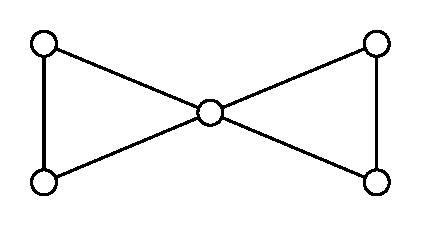
\includegraphics[width=40mm,keepaspectratio]{figures/osszefuggoseg_pelda.pdf}
\caption{Ez a gráf 2-élösszefüggő, de nem 2-összefüggő.}
\label{fig:osszefuggosegek}
\end{figure}

\begin{definicio}[lokális élösszefüggőség]
Az $u$ és $v$ pontok közötti lokális élösszefüggőség ($\lambda(u, v)$) az $u$ és v közötti éldiszjunkt utak maximális száma.
\end{definicio}

\begin{definicio}[lefogó élhalmaz]
A $G$ (irányított vagy irányítatlan) gráf $F$ élhalmaza lefog minden $uv$ utat, ha a $G-F$ gráfban nem létezik $u$-ból $v$-be (irányított) út.
\end{definicio}

Menger tételei alapján:\footnote{BSz2 jegyzet, \url{http://www.cs.bme.hu/~fleiner/jegyzet/}, 1.4.1, Menger tételek, 1. (irányított gráfra) és 3. (irányítatlan gráfra)}

$\lambda(u, v)$ = \{$u$ és $v$ közötti éldiszjunkt utak maximális száma\} = \{$u$ és $v$ közötti utakat lefogó élek minimális száma\}

\begin{allitas}
\[ \lambda(G) = \min_{u, v \in V(G), u \neq v} \lambda(u, v) \]
\end{allitas}

$\lambda(G)$ meghatározása naiv algoritmussal: megvizsgáljuk, hogy adott $k = 1, 2, \ldots$ esetén bármely $k-1$ élt elhagyva $G$ összefüggő marad-e. Ez összesen $\sum_{k=1}^{\lambda(G)} {|E(G)| \choose k-1}$ lépést igényelne. Ezzel szemben a jobb oldalon szereplő kifejezés polinomiális lépésszámban kiértékelhető, pl. folyamok segítségével (ld. később).

\begin{proof} Belátjuk, hogy $\lambda(G) \leq \min \lambda(u, v)$ és $\lambda(G) \geq \min \lambda(u, v)$ is teljesül. 
\begin{itemize}
  \item $\lambda(G) \leq \min \lambda(u, v) = k$: kiválasztjuk azt az $(u, v)$ csúcspárt, amely csúcsok között a minimum felvétetik. A két csúcs között legfeljebb $k$ darab éldiszjunkt út fut, ezeket le tudjuk fogni $k$ éllel. Ezt a $k$ élt törölve $G$ szétesik, $G$ tehát nem lehet $(k+1)$-élösszefüggő, legfeljebb $k$-élösszefüggő.
  
  
  \item $\lambda(G) \geq \min \lambda(u, v) = k$: bármely két pont között van legalább $k$ éldiszjunkt út, ekkor $k-1$ él elhagyásával nem eshet szét a gráf, tehát legalább $k$-élösszefüggő: $\lambda(G) \geq k$.
\end{itemize}
\end{proof}

Egy (esetleg irányított) gráf élösszefüggőségének kiszámítására kézenfekvő a maximális folyam algoritmus használata. A $G$ gráfból olyan hálózatot készítünk, amelyben minden él kapacitása egységnyi. Irányítatlan gráf esetén az éleket irányítjuk: egy irányítatlan $\{a,b\}$ élre a hálózatba $(a,b)$ és $(b,a)$ irányított éleket húzunk. 
Ekkor egy rögzített $u$, $v$ pontpárra a $\lambda(u, v)$ érték éppen az $u$ és $v$ közötti maximális folyam értéke.

A folyamprobléma megoldására a javítóutas Edmonds-Karp algoritmus\footnote{A BSz2 jegyzetben található Edmonds--Karp tétel leírja az algoritmust és kimondja, hogy az polinomiális.} lépésszáma $O(|V| \cdot |E|^2) = O(n^5)$, de létezik kevésbé szemléletes, $O(n^3)$ lépésszámú algoritmus.

\begin{algoritmus}[$\lambda(G)$ meghatározása négyzetes számú folyamkereséssel]
Minden $(u, v)$ párra megvizsgáljuk a folyamértéket, ezek minimuma lesz $\lambda(G)$. Az $(u, v)$ párok száma ${n \choose 2} = \Theta(n^2)$. Az algoritmus lépésszáma $O(n^2 \cdot n^3) = O(n^5)$.
\end{algoritmus}

\begin{algoritmus}[$\lambda(G)$ meghatározása lineáris számú folyamkereséssel] A 

\[ \lambda(G) = \min_{v \in V(G)-a} \lambda(a, v) \]

egyenlőség felhasználásával $\lambda(G)$ értéke $n-1$ folyamprobléma megoldásával, $O(n \cdot n^3) = O(n^4)$ lépésben meghatározható.
\end{algoritmus}

\begin{proof} A négyzetes számú folyamkereséshez képest szűkebb halmazon vizsgálódunk, ezért azt kell garantáltunk, hogy bármely $a$ csúcsból kiindulva a $\lambda(a, v)$ értékek között lesz $\lambda(G)$ értékű. Legyen $k=\lambda(G)$. Nyilván minden $b \in V(G)-a$ csúcsra igaz, hogy 

\[ k = \min_{u, v \in V(G), u \neq v} \lambda(u, v) \leq \min_{v \in V(G)-a} \lambda(a, v) \leq \lambda(a, b), \]

azaz $\lambda(a, b) \geq k$.

Hagyjunk el $G$-ből $k$ élt úgy, hogy szétessen, ekkor a kapott részgráfnak legalább két komponense lesz. Mivel $a$ rögzített, válasszuk ki $b$-t úgy, hogy $a$ és $b$ külön komponensben legyenek, ekkor $\lambda(a, b) \leq k$.

$\lambda(a, b) \geq k$ miatt $\lambda(a,b) = k = \lambda(G)$, azaz lesz olyan $b$ csúcs, ahol a $\lambda(G)$-nek megfelelő minimum felvétetik.

\end{proof}

% ----------------------------------------------------------------------------

\section*{21. tétel}
\begin{framed}
$\lambda(G)$ meghatározása összehúzások segítségével, Mader tétele (biz. nélkül), Nagamochi és Ibaraki algoritmusa (biz. nélkül).
\end{framed}

Nagamochi és Ibaraki megmutatták, hogy egy irányítatlan gráf élösszefüggőségi számát folyamok használata nélkül is ki tudjuk számolni $O(|V(G)|^3)$ lépésben. Az alábbiakban definiáljuk az ehhez szükséges fogalmakat és állításokat.

\begin{figure}
\centering
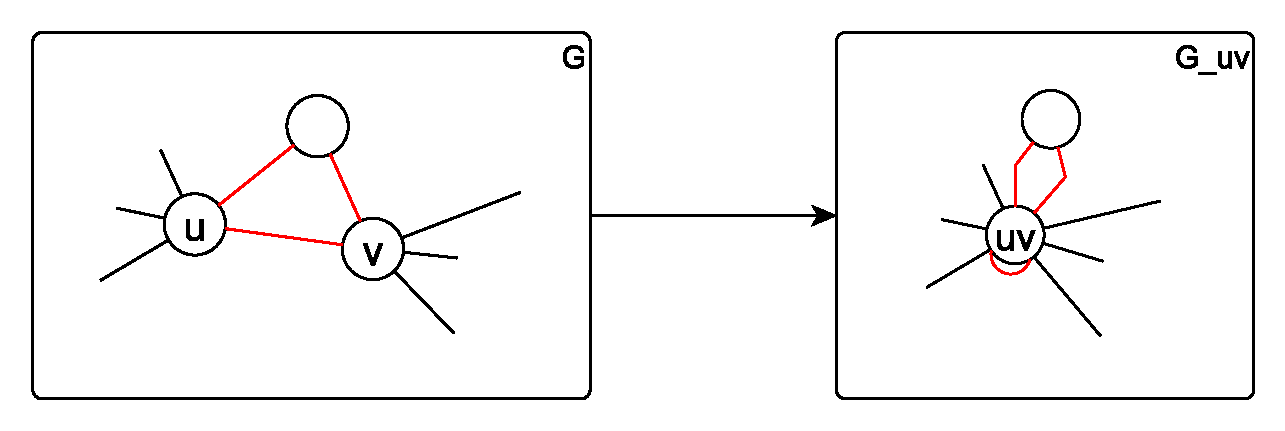
\includegraphics[width=100mm,keepaspectratio]{figures/osszehuzas.pdf}
\caption{Összehúzás}
\label{fig:osszehuzas}
\end{figure}

\begin{definicio}[összehúzás] A $G$ gráf két $u, v$ csúcsát összehúzva olyan $G_{uv}$ gráfot kapunk, amelyben a $G$ gráfban $u$-val vagy $v$-vel összekötött csúcsok az $uv$ csúccsal vannak összekötve. Ha $G$ egy $p$ pontjából $u$-ba és $v$-be is futott él, $G_uv$-ben párhuzamos élek lesznek $p$ és $uv$ között. Ha az összehúzott csúcsok között futott él, $uv$-n hurokél lesz (\ref{fig:osszehuzas}. ábra).
\end{definicio}

\begin{allitas}
A hurokélek nem befolyásolják az élösszefüggőségi számot (ennek bizonyítása triviális).
\end{allitas}

\begin{allitas}
A gráf két pontját összehúzva a minimális vágás mérete nem csökkenhet, sőt, csak akkor nőhet, ha minden minimális vágás elválasztja az összehúzott pontokat. Így érvényes az alábbi egyenlőség:
\[ \lambda(G) = \min(\lambda(u, v), \lambda(G_{uv})) \]
\end{allitas}


\begin{proof}
Belátjuk, hogy $\lambda(G)$ legfeljebb $\lambda(u,v)$, legfeljebb $\lambda(G_{uv})$, és az egyikkel egyenlő is.

\begin{enumerate}
  \item $\lambda(G) \leq \lambda(u, v)$. Triviális a $\lambda(G) = \min_{u, v \in V(G), u \neq v} \lambda(u, v)$ definíció miatt.
  \item $\lambda(G) \leq \lambda(G_{uv}) $\\
  	Ha $G_{uv}$ nem összefüggő, akkor az összehúzás előtt $G$ sem volt az (az állítás megfordítása nem igaz, ha $G$ nem összefüggő, akkor $G_{uv}$ lehet az, pl. egy $C_2$-ből és egy izolált pontból álló gráf esetén a $C_2$ egyik pontját az izolált ponttal összehúzva összefüggő gráfot kapunk).\\
  	$\lambda(G_{uv}) = k$ esetén $G_{uv}$-nek van $k$ olyan éle, amit elhagyva szétesik. A $G_{uv}$-beli vágást $G$-re transzformálva a megfelelő $k$ élt elhagyva $G$ is szétesik, mert ha nem így lenne, akkor az összehúzás utáni $G_{uv}$ is összefüggő lenne. Ezért $\lambda(G) \leq k$ biztosan teljesül, $\lambda(G_{uv}) = k$ miatt $\lambda(G) \leq \lambda(G_{uv})$.
  \item $k = \lambda(G) = \lambda(u,v)$ vagy $\lambda(G) = \lambda(G_{uv})$. Vegyünk egy $k$ élű vágást $G$-ben.
 	\begin{itemize}
      \item Ha a $k$ élt elhagyva $u$ és $v$ különböző komponensben vannak, akkor $\lambda(u, v) \leq k$, azaz $\lambda(u,v) \leq \lambda(G)$. Korábban beláttuk, hogy $\lambda(G) \leq \lambda(u, v)$, tehát $\lambda(G) = \lambda(u, v)$.
      \item Ha ugyanabban a komponensben vannak, akkor $G_{uv}$ is szétesik ugyanannak a $k$ élnek az elhagyásával (mert  $u$ és $v$ összehúzása nem teheti összefüggővé), tehát $\lambda(G_{uv}) \leq k$, azaz $\lambda(G_{uv}) \leq \lambda(G)$. Korábban beláttuk, hogy $\lambda(G) \leq \lambda(G_{uv})$, tehát $\lambda(G) = \lambda(G_{uv})$. 
    \end{itemize}
\end{enumerate}
\end{proof}

\begin{tetel}[Mader-tétel]
Minden $G$ gráfban létezik olyan $u, v \in V(G)$ csúcspár, hogy $\lambda(u,v) = d(v)$.
\end{tetel}

\begin{definicio}[max-vissza sorrend]
A $G=(V,E)$ gráf pontjainak egy $(v_1, \dots, v_n)$ sorrendje max-vissza sorrend, ha minden $i$, $j$ ($2 \leq i < j \leq n$) párra teljesül, hogy
\[ d(v_i, V_i) \geq d(v_j, V_i), \]
ahol $d(a, B)$ az $a$ és a $B$ közötti élek száma, $V_i=\{v_1, \ldots, v_{i-1}\}$.\footnote{A könyvben $V_i = \{v_1, \ldots, v_i\}$, ekkor a feltétel $d(v_i, V_{i-1}) \geq d(v_j, V_{i-1})$-re módosul}

Ilyen sorrend például úgy készíthető, hogy mindig arra ügyelünk, hogy a soron következő pont olyan legyen, amelyből a már sorba rakott pontokhoz a lehető legtöbb él vezet.
\end{definicio}

\begin{tetel}
$\lambda(v_{n-1}, v_n) = d(v_n)$, ahol $v_{n-1}, v_n$ az utolsó két pont $G$ pontjainak egy max-vissza sorrendjében. (Nem bizonyítjuk.)
\end{tetel}

Ha tehát minden iterációban az összehúzandó párt egy max-vissza sorrend utolsó két pontjaként választjuk, a keresett $\lambda(v_{n-1}, v_n)$ érték a $d(v_n)$ fokszám lesz. Így a következő algoritmus helyesen számolja ki egy legalább két pontú gráfra a $\lambda(G)$ értéket. 

\begin{algoritmus}[Nagamochi--Ibaraki] Az algoritmus két lépésből áll:
\begin{enumerate}
  \item Legyen $\lambda = \infty$
  \item Készítsük el a gráf pontjainak egy max-vissza sorrendjét. Ha ebben $d(v_n) < \lambda$, akkor legyen $\lambda = d(v_n)$. Ha még legalább hárompontú a gráf, húzzuk össze a sorrend utolsó két pontját és kezdjük újra a 2. lépést. Ha már csak két pont maradt, $\lambda(G)$ értéke a két pont között futó párhuzamos élek száma, az algoritmus eredménye $\lambda = \lambda(G)$.
\end{enumerate}
\end{algoritmus}

% ----------------------------------------------------------------------------

\section*{22. tétel}
\begin{framed}
Minimális méretű 2-élösszefüggő, illetve 2-összefüggő részgráfok keresése. A problémák NP-nehézsége, Khuller--Vishkin (bizonyítás nélkül, de éles példával) és Cheriyan-Thurimella algoritmusok (biz. nélkül).
\end{framed}

Legyen $G=(V,E)$ egy 2-élösszefüggő irányítatlan gráf, ahol minden él súlya egységnyi. Olyan $G'$ feszítő részgráfot keresünk, melyben minden $u, v \in V(G)$ pontpárra $\lambda(u, v) \geq 2$ és a $G'$ összsúlya minimális. Tehát a feladat egy minimális élszámú 2-élösszefüggő feszítő részgráf keresése $G$-ben.

Az optimum értéke pontosan akkor $|V(G)|$, ha $G$ tartalmaz Hamilton-kört. Mivel a Hamilton-kör keresése visszavezethető erre a problémára, az optimum meghatározása NP-nehéz.

\begin{definicio}[elvágó él]
$e \in E(G)$ elvágó él, ha $G-e$ nem összefüggő.
\end{definicio}

\begin{algoritmus}[Khuller--Vishkin]
Az algoritmus 2-élösszefüggő irányítatlan gráfban 2-élösszefüggő feszítőgráfot keres, approximációs faktora $\frac{3}{2}$ (az ismert legjobb approximációs algoritmusé $\frac{4}{3}$).

A leírás során $E'$ jelöli a megoldáshalmazt. Tetszőleges pontból kiindulva mélységi bejárást hajtunk végre. A keresés során a $T$ mélységi fa minden élét belevesszük $E'$-be. Mindig, amikor a keresés egy $v$ pontból visszalép a $T$ valamelyik $uv$ éle mentén (ekkor a $T$-nek a $v$ pontból gyökerező $T(v)$ részfáját már teljesen bejártuk), ellenőrizzük, hogy az $uv$ él elvágó-e az eddig kijelölt $E'$ élhalmaz által feszített gráfban.\footnote{$uv$ egy visszaél, mert irányítatlan gráfok mélységi bejárása során nincsenek keresztélek. Nem fordulhat elő ugyanis az, hogy egy $uv$ él esetén $u$ mélységi száma nagyobb, mint $v$-é, úgy, hogy $v$ befejezési száma pozitív, mert ekkor az $uv$ él mentén $v$-ből bejártuk volna $u$-t is, így $v$ befejezési száma az él vizsgálatakor 0 lenne. Ld. \url{http://cs.bme.hu/algel/9elo-2012.pdf}, 10--11. dia} Ha igen, akkor az $E'$-höz egy olyan $T(v)$-ből -- tehát nem csak $v$-ből, hanem a $v$-ből kiinduló részfájából -- kilépő élt adunk hozzá, mely nincs $T$-ben és $T(v)$-n kívüli végpontját a keresés először érte el (azaz a mélységi száma a legkisebb).

A végén kapott $E'$ élhalmaz által feszített részgráf lesz az algoritmus kimenete.\footnote{Az algoritmus leírása megtalálható az alábbi cikkben: \url{http://citeseerx.ist.psu.edu/viewdoc/summary?doi=10.1.1.56.8290}. Éles példa a 3.2.3. szakaszban.} Az algoritmus működése \aref{fig:khuller_vishkin_pelda}. ábrán látható.
\end{algoritmus}

\begin{figure}
\centering
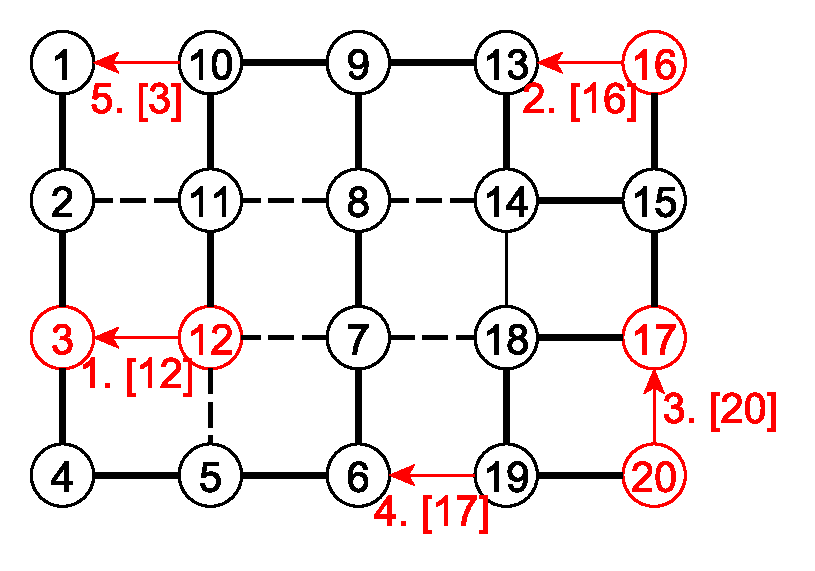
\includegraphics[width=80mm,keepaspectratio]{figures/khuller_vishkin_pelda.pdf}
\caption{A Khuller--Vishkin algoritmus működése. A csúcsok sorszámai a mélységi bejárás során kapott mélységi számok. A vastag fekete élek jelölik a mélységi bejárás útját, a vékony piros élek a visszalépéskor hozzáadott élek (a feliratuk behúzás sorszáma, szögletes zárójelben az a csúcs, amelyből történő visszalépéskor behúztuk), a szaggatott élek az $E \backslash E'$-beli élek.}
\label{fig:khuller_vishkin_pelda}
\end{figure}

\begin{figure}
\centering
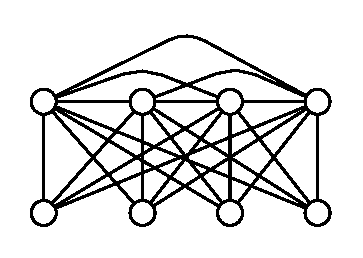
\includegraphics[width=60mm,keepaspectratio]{figures/khuller_vishkin_eles_pelda.pdf}
\caption{}
\label{fig:khuller_vishkin_eles_pelda}
\end{figure}

\begin{figure}
\centering
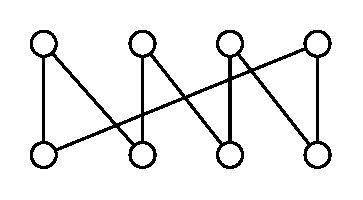
\includegraphics[width=60mm,keepaspectratio]{figures/khuller_vishkin_eles_opt.pdf}
\caption{}
\label{fig:khuller_vishkin_eles_opt}
\end{figure}

\begin{figure}
\centering
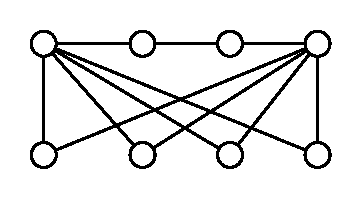
\includegraphics[width=60mm,keepaspectratio]{figures/khuller_vishkin_eles_alg.pdf}
\caption{}
\label{fig:khuller_vishkin_eles_alg}
\end{figure}

\begin{pelda}[Éles példa a Khuller--Vishkin algoritmusra]
$K_{n,n}$ teljes gráf, a gráf egyik partíciójában minden csúcs minden csúccsal össze van kötve, tehát a partíció pontjai által feszített részgráf egy $K_n$ teljes gráf (\ref{fig:khuller_vishkin_eles_pelda}. ábra).

Az optimum $2n$ élű (\ref{fig:khuller_vishkin_eles_opt}. ábra), míg az algoritmus $3n-1$ élű megoldást ad (\ref{fig:khuller_vishkin_eles_alg}. ábra). Egy algoritmus $k$-approximációs, ha minden $I$ bemenetre polinomidőben szolgáltat egy $y \in X_I$ megoldást, amire (minimalizálási probléma esetén) 

\[ f(y) \leq k \min_{x \in X_I} f(x) \]

Az algoritmus által adott megoldást és az optimálisat behelyettesítve:

\[ 3n-1 \leq k \cdot 2n \]

\[ \frac{3n-1}{2n} \leq k \]

\[ \frac{3}{2}-\frac{1}{n} \leq k \]

Tehát az approximációs faktor nem lehet jobb $\frac{3}{2}$-nél.
\end{pelda}

\begin{definicio}
Jelöljük $\nu(G)$-vel a $G$ gráfban található független élek maximális számát, $\rho(G)$-vel a lefogó élek minimális számát.
\end{definicio}

\begin{tetel}[2. Gallai tétel]
$\nu(G)+\rho(G)=|V(G)|$ minden $G$ gráfra, amelyben nincs izolált pont.
\end{tetel}

\begin{proof}
{\it (A bizonyítás nem része a számonkérésnek).}

Az állítás átrendezve: $|V(G)|-\nu(G)=\rho(G)$.

Belátjuk, hogy $|V(G)|-\nu(G)\geq\rho(G)$ és $|V(G)|-\nu(G)\leq\rho(G)$ teljesül. 

\begin{itemize}
  \item Egy $\nu(G)$ elemű $X$ független élhalmaz lefog $2\nu(G)$ különböző pontot. A többi pont (mivel nincs köztük izolált) nyilván lefogható $|V(G)| - 2\nu(G)$ éllel, így összesen $\nu(G) + |V(G)| - 2\nu(G) = |V(G)| - \nu(G)$ éllel biztosan lefogható az összes pont, tehát $|V(G)| - \nu(G) \geq \rho(G)$.
  \item Másrészt, ha $Y$ egy minimális méretű lefogó élhalmaz, akkor $Y$ néhány (mondjuk $k$ darab) diszjunkt csillag\footnote{csillag: olyan fa, amelyet úgy kapunk, ha $l$ csúcsot egyenként összekötünk a központi csúccsal ($K_{1,l}$)}. egyesítése. Ha ugyanis $Y$ tartalmazna kört, akkor annak bármely élét, ha pedig 3 hosszú utat, akkor annak középső élét el lehetne hagyni $Y$-ból, mert a többi él mindig lefogná az összes pontot. Így $\rho(G) = |V(G)|-k$, hiszen a $k$ csillag csúcsainak lefogásához $|V(G)|-k$ él kell (a középpontokat leszámítva minden csúcshoz egy-egy él). Tehát $k=|V(G)|-\rho(G)$.\\Ha minden csillagból kiválasztunk egy élt, az így kapott élhalmaz nyilván független, tehát $\nu(G) \geq k = |V(G)|-\rho(G)$, azaz $\nu(G) \geq |V(G)|-\rho(G)$, így $\rho(G) \geq |V(G)|-\nu(G)$ teljesül. 
\end{itemize}
\end{proof}

\begin{algoritmus}[Cheriyan-Thurimella]
Adott 2-összefüggő $G$ gráfnak meghatározza egy olyan 2-összefüggő feszítő részgráfját, amelyben az optimumnál legfeljebb  $\frac{3}{2}$-szer több él van ($\frac{3}{2}$-approximáció).

\begin{enumerate}
  \item Keressünk egy minimális méretű $L$ lefogó élhalmazt $G$-ben. (Nem csak páros, hanem általános gráfban is készíthetünk maximális párosítást polinomidőben: nem csak {\it maximal}, azaz tovább nem bővíthető, hanem {\it maximum}, azaz maximális méretű párosítás keresésére is létezik hatékony algoritmus.\footnote{Edmonds-algoritmus, ld. \url{http://www.cs.berkeley.edu/~karp/greatalgo/lecture05.pdf}} Egy maximális méretű párosításból kiindulva, a párosításhoz néhány él hozzávételével minimális lefogó élhalmazt kapunk, ld. a Gallai-tétel bizonyítását).  
  \item Hagyjunk el $G$-ből $E \backslash L$-beli éleket amíg csak lehet, úgy, hogy a gráf 2-összefüggő maradjon.
\end{enumerate}

A megmaradó élek által feszített részgráf az algoritmus kimenete.

Az algoritmus működése \aref{fig:cheriyan_thurimella_pelda}. ábrán látható. Az ábrán $|L| = 10$, $E \backslash L$-ben 13 él marad, a kapott feszítő részgráf összesen 23 élből áll.

\begin{figure}[h]
\centering
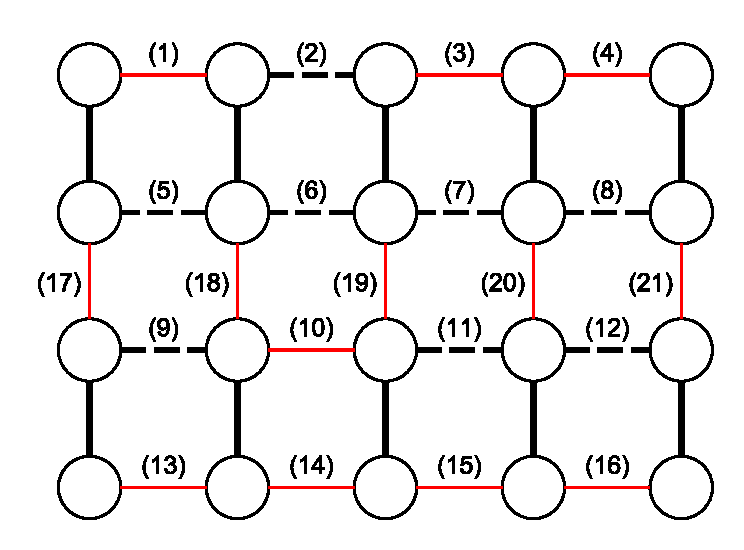
\includegraphics[width=80mm,keepaspectratio]{figures/cheriyan_thurimella_pelda.pdf}
\caption{A Cheriyan--Thurimella algoritmus működése. A vastag fekete élek a minimális lefogó élhalmaz élei, a szaggatott vonallal jelzetteket töröltük, a vékony piros élek maradtak meg az $E \backslash L$ halmazból. A zárójelben lévő számok az egyes élek vizsgálatának sorrendjét jelölik.}
\label{fig:cheriyan_thurimella_pelda}
\end{figure}
\end{algoritmus}

% ----------------------------------------------------------------------------  
  
\end{document}